\chapter{Implementation Broker}
\label{chap:broker}

The broker implementation is a stand-alone server application based on the
Apache Kafka protocol implementation (see \ref{sec-protocol}). To clarify the
program flow from receiving data from the network, handling the requests, and
accessing the message log, the broker is split into three layers, each with its
own module.

\begin{description}
    \item [Network Layer] \hfill \\
        This module encapsulates action on the network. It initiates
        connections and receives bytes from client. It chunks the received bytes
        into single requests and provides it to the API Layer. 
    \item [API Layer] \hfill \\
        This module handles incoming requests. It first parses the
        received bytes as RequestMessage and then proceeds to an appropriate action,
        depending on the delivered API key. After performing the action, an
        according ResponseMessage is generated and provided to the Network Layer
        to send back to the client. 
    \item [Log Layer] \hfill \\
        This module encapsulates actions to the log on the filesystem.
        Fundamental functions are appending MessageSet's to Log or reading from
        it. 
\end{description}

\begin{figure}[H]
    \centering
    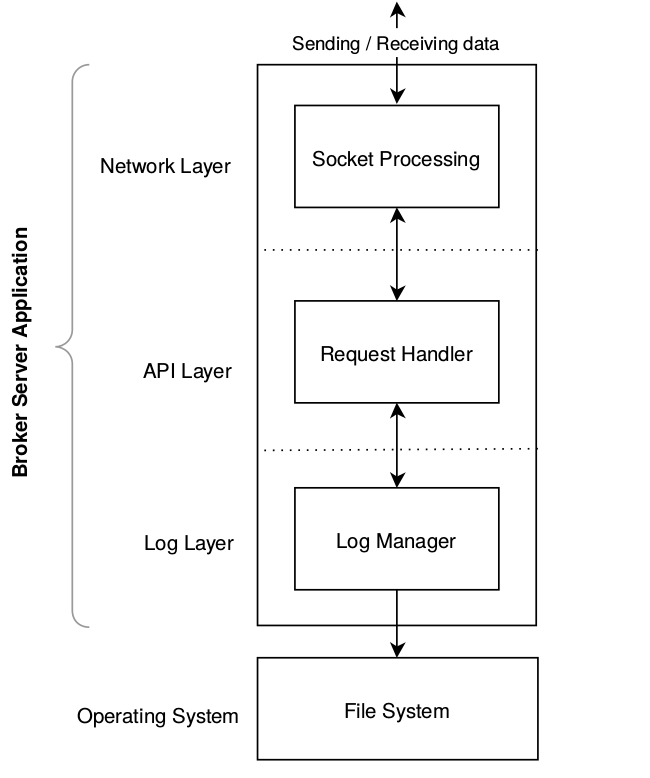
\includegraphics[width=0.45\textwidth]{images/impl-brok-layers.png}
    \caption{Three subsystems of broker server application}
    \label{fig:impl-brok-layers}
\end{figure}

\newpage
\section{Network Layer}
\label{sec:broker-network}

The broker application has a thin network layer which is responsible for
receiving and sending binary data to clients. Instead of using HTTP,
connection-oriented sockets (TCP) are used. Therefore, the broker is independent
from any HTTP implementation, and clients can make use of advanced TCP features
like the ability to simultaneously poll many connections or multiplex requests.
While a socket is an endpoint of a bidirectional inter-process communication
flow, each connection established to the broker is basically a socket
connection. That being said, it is important to provide a reliable socket server
implementation which will serve correctly under a heavy load. Haskell provides
full control over sockets using the
\fnurl{Network.Socket}{https://hackage.haskell.org/package/network-2.3.0.7/docs/Network-Socket.html}
module which exposes the \fnurl{C socket
API}{http://pubs.opengroup.org/onlinepubs/7908799/xns/syssocket.h.html}.

This section shows the basic operations and describes the used libraries in the
network layer. For further details about the threading concept, see section
\ref{sec:impl-broker-threading} 

\subsection{Socket Connection Establishment}
\label{sec:impl-broker-socket-connection}
%The following figure (\ref{fig:broker-activity}) shows the abstract view of how
%the socket connection between a client and the broker establishes so that a
%communication between those two counterparts can proceed.

%\begin{figure}[H]
%    \centering
%    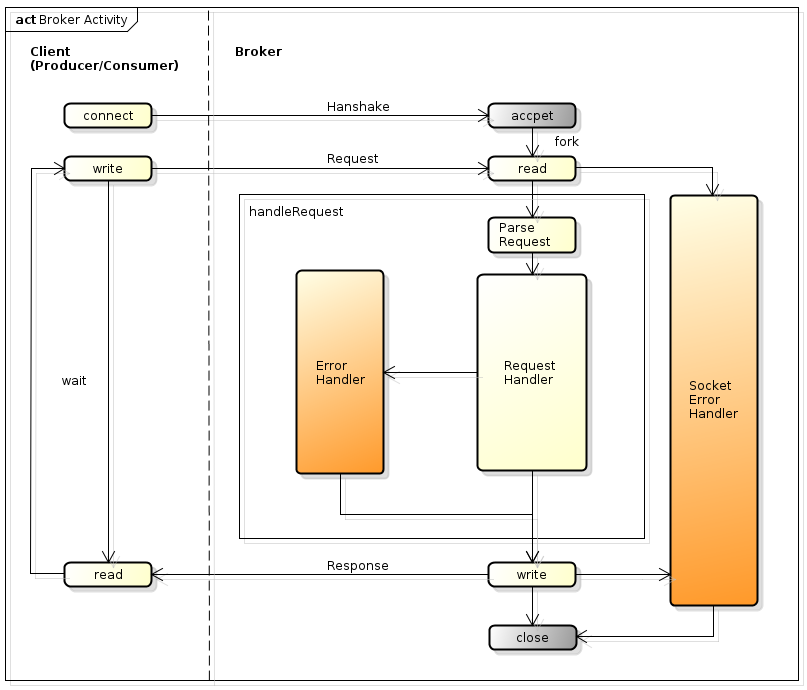
\includegraphics[width=0.7\textwidth]{images/broker-activity.png}
%    \caption{Broker request handling concept}
%    \label{fig:broker-activity}
%\end{figure}

\subsubsection{Initialize Socket}

First of all, the initialization process of a socket happens on the server by providing the following configuration parameters:

\begin{itemize}
    \item {\bf Protocol Family:} \textit{AF\_INET}, for network protocol IPv4.
    \item {\bf Socket Type:} \textit{Stream}, which provides sequenced, reliable, two-way, connection-based byte streams.
    \item {\bf Protocol Number:} \textit{0}, which indicates that the caller does not want to specify the protocol, leaving it up to the service provider.
\end{itemize}

\todo{Socketoption (Send, Recv Buffer, ReuseAddr, etc.)}

\subsubsection{Bind Socket}

After the configuration is set, the socket has to be associated with an address
structure which is a constellation of an IP Address and a Port. The constructor
\textit{SockAddrInet} of data type \textit{SockAddr} takes the following
two arguments:

\begin{itemize}
    \item {\bf Port Number} 4343
    \item {\bf Host Address} iNADDR\_ANY, which binds the socket to all interfaces.
\end{itemize}

\todo{static but could be done with dynamic configuration}

\subsubsection{Listen}

While the socket is created and bound to an interface, the socket state can be
entered into a listening state. The only configuration parameter which has to be
considered is the maximum number of queued connections requesting to
be accepted (also called backlog). While this parameter is not critical in the
constellation of this broker, we set the queue length to \textbf{50} which is
also the default value in the Java SocketServer implementation. \textit{Note
that the focus remains on the amount of data being processed rather than the
number of clients being served.}

\subsection{Receive Data}
\label{sec:impl-broker-socket-receive}
To receive data from the socket buffer, we used the function recv from
\fnurl{Network.Socket.ByteString.Lazy}{https://hackage.haskell.org/package/network-2.3.0.1/docs/Network-Socket-ByteString-Lazy.html}
library which provides access to the Unix socket interface. Because we work
with a binary protocol and need to parse the data from binary data directly,
this module is more efficient than the string based network functions. We
took the lazy variant of the library because the input gets directly parsed by
our lazy based encoder \todo{ref}.

Because we wanted to handle each request individually, we read
the exact amount of bytes needed to get one particular request from
the socket buffer. To get the size of a whole request, we read the first four
bytes, which determines the request size according to the protocol, and parsed it
to an numeral value.

\begin{lstlisting}[caption={Receiving data from socket}]
import qualified Network.Socket.ByteString.Lazy as S 
import qualified Data.ByteString.Lazy as BL

recvFromSock :: (Socket, SockAddr) -> IO BL.ByteString
recvFromSock (sock, sockaddr) =  do 
    respLen <- S.recv sock (4 :: Int64
    let parsedLen = getLength respLen
    req <- recvExactly sock parsedLength 
    where
        getLength = runGet $ fromIntegral <$> getWord32be
\end{lstlisting}

After getting the size of a particular request, this determined amount of bytes
is received from the socket. Because of the blocking semantics of Unix sockets
and TCP packet fragmentation, it is not guaranteed that the len argument for the
recv system call gets exactly the number of bytes of the whole request. The call
may produce less data than specified. Therefore, we implemented the following
function to get the data in chunks until the entire request is read. 

\begin{lstlisting}[caption={Receive exactly amount of bytes}]
recvExactly :: Socket -> Int64 -> IO BL.ByteString 
recvExactly sock size = BL.concat . reverse <$> loop [] 0 
  where
    loop chunks bytesRead
        | bytesRead >= size = return chunks
        | otherwise = do  
            chunk <- S.recv sock (size - bytesRead)
            if BL.null chunk 
              then return chunks 
              else loop (chunk:chunks) $! bytesRead + BL.length chunk 
\end{lstlisting}

\subsection{Send Data}
\label{sec:impl-broker-socket-send}

For every processed request, an appropriate response is sent back to the client.
The actual message is already provided as binary data from the API layer. The
network layer simply needs to send the bytes over the existing connection back
to the client. For sending data over the socket, function sendAll from
\fnurl{Network.Socket.ByteString.Lazy}
{https://hackage.haskell.org/package/network-2.3.0.1/docs/Network-Socket-ByteString-Lazy.html}
is used. This function continues to send data until either all data has been
sent or an error occurs. For further details about Error Handling, see section
\ref{}

\begin{lstlisting}[caption={Send data via socket}]
import qualified Data.ByteString.Lazy as B
import qualified Network.Socket.ByteString.Lazy as S

sendResponse :: (Socket, SockAddr) -> B.ByteString -> IO (Either IOError ())
sendResponse (socket, addr) responsemessage = 
             try(S.sendAll socket responsemessage) :: IO (Either IOError ())
\end{lstlisting}

\newpage
\section{API Layer}
\label{sec:broker-api}

This part of the broker is a quite thin layer which basically handles incoming
requests, initiates any actions needed, and prepares appropriate responses. It
fulfills the essential part in error handling which is described in section
\ref{sec:broker-error-handling}. 

\subsection{Decode Request}
\label{sec:impl-broker-api-handle}

After getting the next bytestring from \lstinline{RequestChan} (see threading
concept in section \ref{sec:impl-broker-threading}), the incoming request first
gets decoded. For this part, the API layer simply uses functions provided by the
protocol implementation (see chapter \ref{sec-protocol}).

\subsection{Handling Requests}

The main focus of the API layer lies on handling the requests properly.
Depending on the API key field of type \lstinline{RequestMessage}, the request
handler determines an appropriate action. In case of a valid API key, the
encoded response message is passed back to the Network Layer via
\lstinline{ResponseChan}.

For nearly all provided APIs, the broker needs access to the functions provided
by the log subsystem as described in section \ref{sec:impl-broker-log}.
Therefore, the API layer initializes the LogManager and passes it to the
handling function below:

\begin{lstlisting}[caption={Handling requests depending on ApiKey}]
handleRequest :: RequestMessage -> LogManager.State 
                 -> IO (Either HandleError BL.ByteString)
handleRequest rm = do
   handle <- case rqApiKey rm of
    0  -> handleProduceRequest rm
    1  -> handleFetchRequest rm
    2  -> handleOffsetRequest rm
    3  -> handleMetadataRequest rm
    8  -> handleOffsetCommitRequest rm
    9  -> handleOffsetFetchRequest rm
    10 -> handleConsumerMetadataRequest rm
    _  -> return (Left UnknownRqError)
   return handle
\end{lstlisting}

\newpage
\subsubsection{HandleProduceRequest}
\label{subsec:broker-api-producerequest}

Handling a produce request implies that the API layer passes the containing
messages to the append function provided by the \lstinline{LogManager}. A
request may contain messages for multiple topics or partitions, and each
combination refers to another log file. Therefore, the job of the API layer is
unnesting the request into single calls to the \lstinline{LogManager}.

\begin{verbatim}
Simplified structure of nested sequences in request:
[Topic [Partition [M]]]

Example:
[TopicA [Part0 [M], Part1 [M]], Topic B [Part0 [M]]]

Unnested to three tuples which can be feed to LogManager as a single call each:
[(TopicA, Part0, [M]), (TopicA, Part1, [M]), (TopicB, Part0, [M])]

\end{verbatim}

Thanks to Haskell's list comprehension, the unnesting of the request can be made
elegant:

\begin{lstlisting}[caption={Handling produce request}]
[(s, BC.unpack(rqToName x)
  , fromIntegral(rqPrPartitionNumber y)
  , rqPrMessageSet y ) 
  | x <- rqPrTopics req, y <- rqToPartitions x
]
\end{lstlisting}

\subsubsection{HandleFetchRequest}
\label{subsec:broker-api-fetchrequest}

Analog to the produce request, handling a fetch request leads to an according
\lstinline{readLog} call on the \lstinline{LogManager}. The retrieved messages
are packed and encoded to a protocol conform fetch response.

Fetching data for multiple topics or partitions is not yet supported.

\subsubsection{HandleMetadataRequest}

Handling a request to the metadata API includes gathering information on the
broker system and provided topics and packing them to a metadata response.
Getting replication and partition related information is not yet implemented.

For retrieving a list of provided topics, the \lstinline{LogManager} is again
involved. The exposed function \lstinline{getTopicNames} analyses the existing
file structure and gives the available topics.

Information regarding the broker host includes local IP. Therefore, the library
\fnurl{Network.Info}{https://hackage.haskell.org/package/network-info} is used:

\begin{lstlisting}[caption={Get broker's host adress}]
import qualified Network.Info as N
getHost :: IO N.NetworkInterface
getHost = do
  ns <- N.getNetworkInterfaces
  return $ head $ 
        filter ((N.NetworkInterface name ipv4 ipv6 mac) -> name == "eth0") ns
\end{lstlisting}

\newpage
\section{Error Handling}
\label{sec:broker-error-handling}

A message broker relies fundamentally on error handling, as fault tolerance and
reliability are key requirements of such a system. The first part of this
section concentrates on the architectural details and decisions made regarding
error handling. Using a demonstration of a message flow, possible edge cases are
considered and uncovered in order to provide reliability to the user of this
broker. The second part covers the techniques used in Haskell to handle the
previously described concept and cases where errors may occur. It will also
involve part of the concept behind the error handling of Apache Kafka, which is
partly integrated in the Apache Kafka Protocol and thus adapted in this
implementation.

\subsection{Message Flow}

Figure (\ref{fig:broker-error-activity}) provides insight into the process that
an incoming request message goes through. For simplicity, one may think of a
message proceeding through all steps successively. But in fact, multiple
requests are handled at the same time. Assuming the connection to the broker is
established and the client is ready to send requests to the broker, there are
principally two types of errors that may occur for each, which there is a
separate handler to handle errors appropriately.

\begin{figure}[H]
  \centering
  \resizebox {0.7\linewidth} {!} {
    \begin{tikzpicture}[node distance=1cm, font=\small\sffamily]
%------------------------------------------------------
%Draw elements
%------------------------------------------------------
\node (connect) [block] {connect};
\node (write) [block, below of=connect] {write};
\node (read) [block, below of=write, yshift=-8cm] {read};
\node (accept) [block, right of=connect, xshift=6cm] {accept};
\node (read1) [block, below of=accept] {read};
\node (preq) [block, below of=read1, yshift=-1cm] {Parse Request};
\node (hreq) [block, below of=preq, yshift=-2cm, minimum height = 4cm] {Request Handler};
\node (errh) [block, left of=hreq, xshift=-2cm, minimum height = 4cm, text width=1.5cm] {Request Error Handler};
\node (write1) [block, below of=hreq, yshift=-3cm] {write};
\node (close) [block, below of=write1, yshift=-.5cm] {close};
\node (serrh) [block, right of=hreq, xshift=2.5cm, minimum height = 9cm, text width=2cm] {Socket Error Handler};
%------------------------------------------------------

%------------------------------------------------------
%Draw rectangles and text
%------------------------------------------------------
%\node (a) [draw,fit={($(preq.north east)+(.5,.7)$) ($(errh.south west)+(2.4,-.2)$)}] {};
%\node [anchor=north west,inner sep=1pt] at (a.north west) {handle request};
\node (b1) [blank, above of=connect, xshift=-.8cm] {\bfseries{Client\\ (Producer/Consumer)}};
\node (b2) [blank, right of=b1, anchor=south, xshift=7cm] {\bfseries{Broker}};
%\node (b) [draw, fit={($(b1.north west)+(-1,1)$) ($(serrh.south east)+(1,-1.5)$)}] {};
%\node (c) [xshift=-3cm, inner sep=2pt] at (b.south) {}; 
%\node (d) [xshift=-3cm, inner sep=2pt] at (b.north) {};
%\draw [dashed] (c) -- (d);
\node (phantom) [right of=write1, xshift=1.5cm] {};
%------------------------------------------------------

%------------------------------------------------------
%Draw lines between elements
%------------------------------------------------------
\begin{scope}
%Straight lines
\path [line] (connect) -- node[anchor=south]{Handshake} (accept);
\path [line] (write) -- node[anchor=east]{wait} (read);
\path [line] (write) -- node[anchor=south]{Request} (read1);
\path [line] (accept) -- node[anchor=west] {fork} (read1);
\path [line] (read1) -- (preq);
\path [line] (preq) -- (hreq);
\path [line] (hreq) -- (errh);
\path [line] (hreq) -- node [anchor=west, yshift=.3cm] (mid) {} (write1);
\path [line] (write1.east) -- (phantom);
\path [line] (write1) -- node[anchor=south]{Response} (read);
\path [line] (write1) -- (close);
%Angled lines
\path [line] (read1) -| (serrh);
\path [line] (serrh) |- (close);
\path [line] (read) -- + (-2,0) |- (write);
\path [draw] (errh.south) |- (mid);
\end{scope}
%------------------------------------------------------
\end{tikzpicture}

  }
  \caption{Broker error handling concept}
  \label{fig:broker-error-activity}
\end{figure}

\subsubsection{Socket Error}

During the process of listening to an open connection and reading an incoming
byte-stream, as described in \ref{sec:broker-network}, there is a chance of
unexpected errors occuring. In this case, the underlying C socket implementation
will return a result of \textit{-1} which will then result in
an\fnurl{IOError}{https://hackage.haskell.org/package/base-4.4.1.0/docs/System-IO-Error.html}. 

Errors at this stage will be handled using the \textit{Socket Error Handler} and
do not result in any response to the client who initiated the request that
resulted in an error, as the socket connection may be broken. Instead, the error
is simply caught and reported using a separate logging framework such as
\fnurl{hslogger}{https://hackage.haskell.org/package/hslogger}. At worst, the
socket connection is closed.

\subsubsection{Request Error}

One step further in the API-Stage, (\ref{sec:broker-api}) past where socket
errors may occur, the heavy part of error handling begins. For each step, the
request passes may result in an error. To name a few, this can be the case
starting by parsing the request,  writing data to the disk executed by the log
subsystem, or at last producing the response message. All of the mentioned cases
and others who fall into the related category will be handled by the
\textit{RequestErrorHandler}, where a set of possible errors or category of
error is defined, resulting in an appropriate response message sent to the
client.

\subsection{Defining Error Types}

The previously introduced concept of the two error handlers, each responsible
for a certain layer of the application, can be built in Haskell conveniently by
using the \fnurl{Either
Monad}{https://hackage.haskell.org/package/category-extras-0.52.0/docs/Control-Monad-Either.html}
and pattern matching of custom defined error types. This will allow taking
actions based on the given error type.

Error types related to the networking layer are simply distinguished between an
error occurring either in the receiving or responding process.

\begin{lstlisting}[caption={SocketError type}]
data SocketError =
      SocketRecvError String
      | SocketSendError String
      deriving Show
\end{lstlisting}

Any further details are not separated by sub-types. Instead, they can be
described in the first argument of the \lstinline{SocketError}, namely a
\lstinline{String}.

To handle errors during the process of request handling, the data type
\lstinline{HandleError} contains specific types for each edge case in any part
of the application. Those types can be considered as an interface for errors
between the request handler and the underlying subsystems. They are not known to
any subsystem at all but are known to the request handler.

\begin{lstlisting}[caption={Handle Error type}]
data HandleError =
        PrWriteLogError Int String
      | PrPackError String
      | ParseRequestError String
      | FtReadLogError Int String
      | SendResponseError String
      | UnknownRqError
        deriving Show
\end{lstlisting}

\subsection{Error Handlers}

With the knowledge about the types they are related to, either socket or request
errors, it is now possible to create handler functions. They act as a central
place where any kind of error can be sent and will provide the functionality to
appropriately handle. Figure \ref{fig:broker-error-activity-detail} illustrates
that the two mentioned error handlers distinguish their next action based on the
data type containing its arguments that is sent to the error handler.

\begin{figure}[H]
  \centering
  \resizebox {0.7\linewidth} {!} {
    \begin{tikzpicture}[node distance=1cm, font=\small\sffamily]
%------------------------------------------------------
%Draw elements
%------------------------------------------------------
\node (connect) [block] {connect};
\node (write) [block, below of=connect] {write};
\node (read) [block, below of=write, yshift=-8.5cm] {read};
\node (accept) [block, right of=connect, xshift=6.5cm] {accept};
\node (read1) [block, below of=accept] {read};
\node (preq) [block, below of=read1, yshift=-1cm] {Parse Request};
\node (hpreq) [block, below of=preq, yshift=-1cm, text width = 2.5cm] {handleProduce Request};
\node (hfreq) [block, below of=hpreq, yshift=-0.5cm, text width = 2.5cm] {handleFetch Request};
\node (dots) [block, below of=hfreq, yshift=-0.5cm, text width = 2.5cm, minimum height=.8cm] {\ldots};
\node (perr) [block, left of=preq, xshift=-2.5cm, yshift=-0.5cm] {Parse Error};
\node (prrq) [block, left of=hpreq, xshift=-2.5cm] {PrRq Error};
\node (ftrq) [block, left of=hfreq, xshift=-2.5cm] {FtRq Error};
\node (dots1) [block, left of=dots, xshift=-2.5cm] {\ldots};
\node (write1) [block, below of=dots, yshift=-1.5cm] {write};
\node (close) [block, below of=write1, yshift=-0.5cm] {close};
\node (recverr) [block, right of=read1, xshift=3cm, yshift=-1.5cm] {Recv Error};
\node (serr) [block, right of=write1, xshift=3cm] {Send Error};
%------------------------------------------------------

%------------------------------------------------------
%Draw rectangles and text
%------------------------------------------------------
\node (a) [draw,fit={($(perr.north west)+(-.2,.5)$) ($(dots1.south east)+(.2,-.5)$)}] {};
\node [anchor=north west,inner sep=1pt] at (a.north west) {handleHandlerError};
%\node (b) [draw,fit={($(hpreq.north west)+(-.2,.5)$) ($(dots.south east)+(.2,-.5)$)}] {};
\node (c) [draw,fit={($(recverr.north west)+(-.2,.5)$) ($(serr.south east)+(.2,-.5)$)}] {};
\node [anchor=center,inner sep=1pt, text width=2cm] at (c.center) {handle\\ SocketError};
\node (b1) [blank, above of=connect, xshift=-.5cm] {{\bfseries Client\\ (Producer/Consumer)}};
\node (b2) [blank, right of=b1, anchor=south, xshift=7.5cm] {\bfseries{Broker}};
%\node (d) [draw, fit={($(b1.north west)+(-1,1)$) ($(serr.south east)+(1,-2)$)}] {};
%\node (e) [xshift=-3.5cm, inner sep=2pt] at (d.south) {}; 
%\node (f) [xshift=-3.5cm, inner sep=2pt] at (d.north) {};
%\node (ctext) [draw, rectangle, anchor=north west, inner sep=1pt] at (d.north west) {{\bfseries act} Broker Activity};
%\draw [dashed] (e) -- (f);
%\node (g) [draw,fit={($(a.north west)+(-.2,.5)$) ($(b.south east)+(.2,-.5)$)}] {};
%\node [anchor=north west,inner sep=1pt] at (g.north west) {handle request};
%------------------------------------------------------

%------------------------------------------------------
%Draw lines between elements
%------------------------------------------------------
\begin{scope}
%Straight lines
\path [line] (connect) -- node[anchor=south]{Handshake} (accept);
\path [line] (write) -- node[anchor=east]{wait} (read);
\path [line] (write) -- node[anchor=south]{Request} (read1);
\path [line] (accept) -- node[anchor=west] {fork} (read1);
\path [line] (read1) -- (preq);
\path [line] (preq) -- (hpreq);
\path [line] (hpreq) -- (hfreq);
\path [line] (hpreq) -- (prrq);
\path [line] (hfreq) -- (dots);
\path [line] (hfreq) -- (ftrq);
\path [line] (dots) -- node [anchor=west] (mid) {} (write1);
\path [line] (dots) -- (dots1);
\path [line] (write1) -- (serr);
\path [line] (write1) -- node[anchor=south]{Response} (read);
\path [line] (write1) -- (close);
%Angled lines
\path [line] (read1) -| (recverr);
\path [line] (read) -- + (-2,0) |- (write);
\path [draw] (dots1.south) |- (mid);
\path [line] (preq.west) -- +(-.5,0) |- (perr.east);
\path [line] (serr) |- (close);
\end{scope}
%------------------------------------------------------
\end{tikzpicture}
 

  }
  \caption{Broker error handling concept in detail}
  \label{fig:broker-error-activity-detail}
\end{figure}

Assume during the process of an incoming \lstinline{ProduceRequest}, the log
subsystem fails to write data to the disk and returns a log specific error. This
error will not be handled directly. Instead, it is caught by the request handler
(API layer) who is now in charge to map this error to one of the defined
\lstinline{HandleError}. In this specific example, the request handler takes the
error response from the log system, maps it to a \lstinline{String} (if it is
not already mapped) as well as the offset of the failing message, and assigns
this information to the type \lstinline{PrWriteLogError} as the first and second
argument. \\

The following part of this section will describe the functionalites of the
\textit{Socket Error Handler} as well as the \textit{Request Error Handler}
provided by the functions \lstinline{handleSocketError} and
\lstinline{handleHandlerError}.

\subsubsection{Socket Error Handler}

The scope of handling a socket related error is very limited, due to the fact
that the connection may be broken or the client will not receive any more data
using the current connection. Given this, the current implementation only
prints the occurred error on console:

\begin{lstlisting}[caption={Catching error of type SocketError}]
handleSocketError :: (Socket, SockAddr) -> SocketError -> IO()
handleSocketError (sock, sockaddr) (SocketRecvError e) = do
  putStrLn $ "[Socket Receive Error] " ++ e
handleSocketError (sock, sockaddr) (SocketSendError e) = do
  putStrLn $ "[Socket Send Error] " ++ e
\end{lstlisting}

While further logging of errors is out of scope within this thesis, the given
architecture may very well be able to do so. At the point after the pattern
matched--currently implements a \lstinline{putStrLn}--one
could inject an external logging service providing more meaningful information
such as proposed in \fnurl{RFC5424}{http://tools.ietf.org/html/rfc5424}.

\subsubsection{Request Error Handler}

The Apache Kafka Protocol defines error codes (see
\ref{subsec:protocol-types-error-codes}), which should be applied to a response
message if the given failed for some reason. Thus, the
\lstinline{handleHandlerError} function is responsible to provide the related
response message containing the appropriate error code. However, the current
implementation does not suppport a response message caused by an error. Instead,
it prints a notification on the broker side as shown in the code below:

\begin{lstlisting}[caption={Catching error of type HandleError}]
handleHandlerError :: (Socket, SockAddr) -> HandleError -> IO()
handleHandlerError (s, a) (ParseRequestError e) = do
    putStrLn $ (show "[ParseError]: ") ++ e
    putStrLn $ "***Host " ++ (show a) ++ " disconnected ***"
handleHandlerError (s, a) (PrWriteLogError o e) = do
    putStrLn $ show "[WriteLogError on offset " ++ show o ++ "]: " ++ show e
handleHandlerError (s, a) UnknownRqError = do
    putStrLn $ show "[UnknownRqError]"
handleHandlerError (s, a) e = do
    putStrLn $ show e
    S.sendAll s $ C.pack $ show e
    sClose s
    putStrLn $ "***Host " ++ (show a) ++ "disconnected ***"
\end{lstlisting}


\section{Threading}
\label{sec:impl-broker-threading}
The threading concept of the broker server application include the following
instances: 

\begin{description}
\item[Acceptor Thread (one instance)] \hfill \\
    This thread accepts new socket connections (see
    \ref{sec:impl-broker-socket-connection}). To support multiple connections from
    different clients, it forks a new thread for processing incoming data
    whenever a new connection is established. 

\item[Connection Processor Thread (one instance per connection)] \hfill \\
    The incoming socket data needs to be processed as fast as possible. If the
    limit of the socket buffer is reached, the throughput on the network drops
    dramatically. The processor thread constantly receives request
    from a specific connection (see \ref{sec:impl-broker-socket-receive}) and
    provides it to the API handler thread. If the connection is closed, the
    thread will return. 

\item[Responder Thread (one instance per connection)] \hfill \\
    This thread works off the provided responses and sends them back to the original
    client (see \ref{sec:impl-broker-socket-send}). \todo{actually only one
    instance at the moment} \item [API Handler Thread (one to N instances)] \hfill
    \\
    The API handler is a worker thread which works off the received request. It
    also builds appropriate responses and provides it to the responder thread
    (see \ref{sec:impl-broker-api-handle}). It is conceivable to run more than
    a single instance of the API handler. Due to advanced synchronisation, this is
    not realized yet.
\item [Main Thread (one instance)] \hfill \\
    The main function of the broker bootstraps the whole server application. It first
    initializes the network socket and forks the acceptor and API
    handler threads. Threads are managed with the \textit{withAsync} function of
    the \fnurl{Control.Concurrent.Async}
    {https://hackage.haskell.org/package/async-2.0.0.0/docs/Control-Concurrent-Async.html}
    library. It adds a thin layer over the basic concurrency operations provided
    by \fnurl{Control.Concurrent}
    {https://hackage.haskell.org/package/base-4.5.0.0/docs/Control-Concurrent.html}
    and gives the ability to wait for the return value of a thread. This
    provides additional safety and control if a thread crashes. 
\end{description}

Original Apache Kafka has a fix and configurable amount of threads handling
network requests by working with thread pools. Thanks to the optimizations of
the GHC IO manager, the communication with the Haskell threads and the OS is
very efficient due to thread multiplexing. Thread pooling has no further
advantages than one socket processor thread instance per connection. 

For transfer of data between the threads, channels are implemented. The
\fnurl{Control.Concurrent.Chan}
{http://hackage.haskell.org/package/base-4.8.0.0/docs/Control-Concurrent-Chan.html}
package provides a one-way FIFO communication channel. This concept is used to
separate the three layers from each other. The fact that \textit{chan} is
unbounded brings a risk. While \textit{writeChan}--which is being used to write
to a channel--succeeds immediately, there is a chance that the consuming thread
is not able to read the same amount of data in a given time and thus the channel
will grow in an unchecked manner.  \cite{o2008real}

To isolate the network layer from any build or parse process, the transfered
data is type ByteString. Because the response to a particular request needs to
be sent back over the right connection, every chunk of ByteString holds its
corresponding socket connection information in a tuple:

\begin{lstlisting}[caption={Initialize channels for threading}]
import qualified Data.ByteString.Lazy as B

type ChanMessage = ((Socket, SockAddr), B.ByteString)
type RequestChan = Chan ChanMessage
type ResponseChan = Chan ChanMessage
\end{lstlisting}

TODO: sanctions? do we have to block the producer for a short time? ->
Considerations Bounded Chans

\begin{figure}[H]
    \centering
    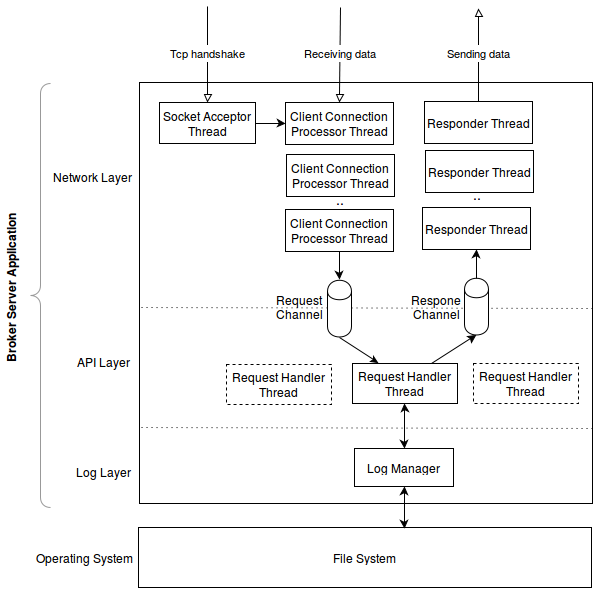
\includegraphics[width=0.85\textwidth]{images/impl-brok-threading.png}
    \caption{Threading concept which channeling}
    \label{fig:impl-brok-threading}
\end{figure}

\newpage
\section{Log Subsystem}
\label{sec:impl-broker-log}

The log subsystem is responsible for the persistence of messages produced and
consumed. This component plays a decisive role while handling a
\textit{fetchRequest} (\ref{subsec:broker-api-fetchrequest}) as well as a
\textit{produceRequest} (\ref{subsec:broker-api-producerequest}). Thus, it is
used extensively in the API layer (\ref{sec:broker-api}). In this section the
applied concepts--which are adapted from Apache Kafka--will be explained before
a proper introduction to the components of the log subsystem is given.
Afterwards follows a code explanation for the most important functionalities,
where information about design decisions and potential threats are given.

\subsection{Components}

Even if the log subsystem lives within the broker environment, it is, from an
architectural point of view, fully decoupled and relies only on the protocol
library.

\begin{figure}[H]
    \centering
    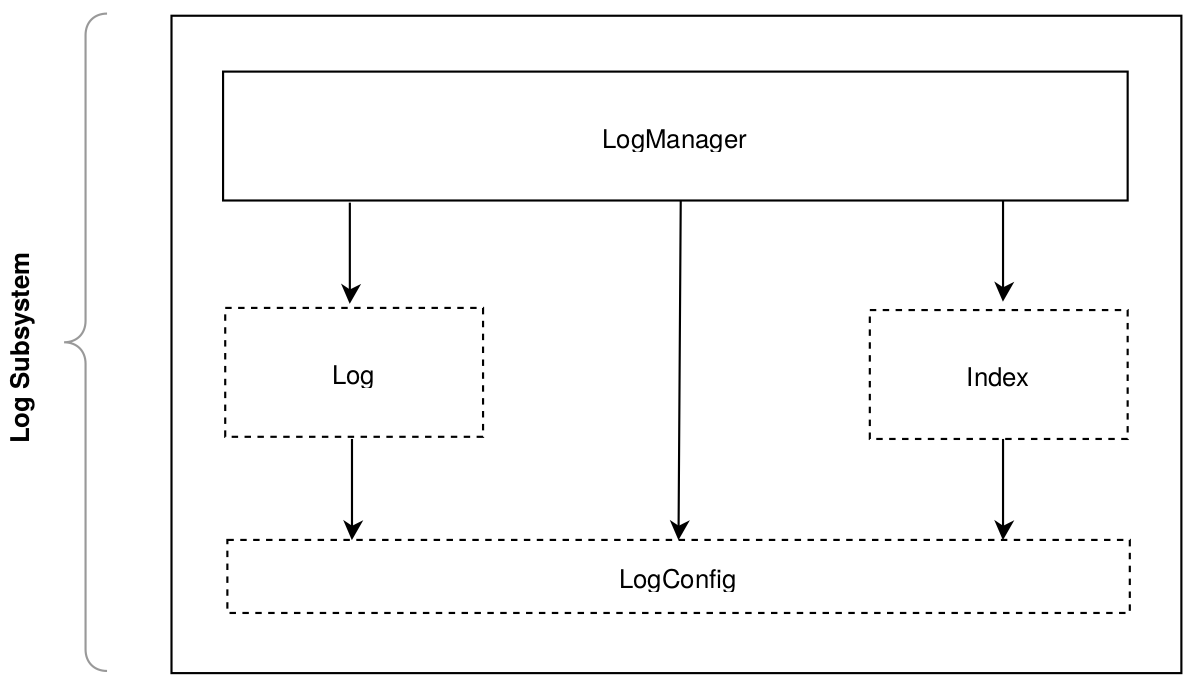
\includegraphics[width=0.65\textwidth]{images/broker-log-overview.png}
    \caption{Architecture of Log Subsystem}
    \label{fig:broker-log-overview}
\end{figure}

As illustrated in figure \ref{fig:broker-log-overview}, the \textit{LogManager}
acts as an interface to any component that uses functionalities of the log,
which in this case will be the API layer. The \textit{LogManager} is then able
to use exposed functionalities of the hidden modules \textit{Log} and
\textit{Index} (displayed as dashed). 

\begin{lstlisting}
module HMB.Internal.LogManager
( new
, append
, readLog
, State
) where
\end{lstlisting}

As for now, the functionalities \textit{LogManager} provides creates a new log
and appends or reads messages to/from an existing log. Further functionalities
are provided but are still managed by the \textit{Log} or \textit{Index} module
itself. Also exposed is the \lstinline{State} type which is the representation
of the current Log and Index, as discussed later in this section.

\newpage
\subsection{Storage Layout}
\label{log-broker-storage}

The storage layout is exactly the same as the one defined for Apache Kafka (see
\ref{intro-kafka-log}).  As for now, the root location of the log is not
configurable and set to the folder named \textbf{./log} within the installation
directory of the broker. Each folder represents a partition of a specific topic,
whereas the name of the folder is a combination of the topic name and the
partition number.

There are two types of files that reside within the folder specifying the
topic and partition (see folder structure):
\begin{itemize}
    \item {\bf .log}: Containing a sequence of log entries as binary data
    \item{\bf .index}: Containing a sequence of index entries as binary data
\end{itemize}

Instead of holding only one storage file per topic-partition combination, the
log can be segmented into multiple files due to reasons of lookup optimization.
Apache Kafka starts segmenting a log after it reaches a configurable size of one
gigabyte. Because of this, both file types hold the same name which stays for
the base offset and can be considered as an unique identifier representing a 64
bit integer as a 20 character file name. As it was defined for Apache Kafka, the
\textbf{base offset} is the offset of the first log entry stored in a file.  For
example if a log holds messages in where the first message has the offset,
\textit{5 :: Int64} the file name of this log will be
\textit{00000000000000000005.log} and the related index file
\textit{00000000000000000005.index}.

Using this naming convention and by viewing multiple log files, one can extract
information about what range of messages reside in which log. This is a very
efficient way to perform a lookup which is needed to append new log messages or
archive old messages.

The following example shows a storage layout for topics \textit{TopicA, TopicB
and TopicC} with the partitions \textit{0} and \textit{1}. Partition 0 of topic
A and B are already segmented into two combinations of an index and log file.

\begin{verbatim}
log
|
+--TopicA_0
   |--00000000000000000000.index
   |--00000000000000000000.log
   |--00000000000008650021.index
   |--00000000000008650021.log
+--TopicA_1
   |--00000000000000000000.index
   |--00000000000000000000.log
+--TopicB_0
   |--00000000000000000000.index
   |--00000000000000000000.log
   |--000000000000128655021.index
   |--000000000000128655021.log
+--TopicB_1
   |--00000000000000000000.index
   |--00000000000000000000.log
+--TopicC_0
   |--00000000000000000000.index
   |--00000000000000000000.log
\end{verbatim}

\newpage
\subsection{Log}

The log contains a sequence of log entries, whereas the on-disk format of a log
entry is part of the reason why the Apache Kafka becomes valuable. In fact, the
on-disk format is exactly the same as the format of the MessageSet (see
\ref{impl-protocol-types-data}) transmitted with a ProduceRequest
(\ref{subsec:protocol-types-producerequest}). Thus, data does not have to be
modified in any way and can directly be extracted and written to the file
system.

\subsection{Index}

Every segment of a log has its corresponding index represented as a file with
the suffix \textit{.index}. Whereas the log file contains the actual messages
structured in a message format (see \ref{impl-protocol-types-data}) and for each
message within this file, the first 64 bits describe the incremented offset.
Looking up this file for messages with a specific offset becomes very expensive
since log files may grow in the range of gigabytes. And to be able to produce
messages, the broker actually has to do such kind of lookups to determine the
latest offset and be able to further increment incoming messages correctly. This
is why there is an index.

Basically, the index file contains simple entries with the following
structure:

\begin{verbatim}
    Relative Offset (4 Bytes)
    Physical Position (4 Bytes)
\end{verbatim}

The first field of an index entry, the relative offset, refers to a specific
message in the corresponding log file. On the other hand, the second field
represents the physical position of the refered message within the log file.
Instead of storing the whole eight bytes of the message offset, the index entry
only holds a relative offset to the base offset. This obviously reduces the size
of the index. In addition, there is to note that not every message within the
log is going to be indexed. By default, an index entry is created only after
\textit{4096 Bytes} of log data.

\subsubsection{Usage and advantages}

As per protocol specification, the request to fetch messages (see
\ref{subsubsec:protocol-fetchrequest}) holds the offset of the wanted message.
Given this offset, one can determine the base offset and is discussed later in
the log section (see \ref{subsubsec:broker-log-general-baseoffset}).  Assuming
to have a valid base offset as well as the actual offset of the requested
message, it is not a big deal to figure out the relative offset of this message:

\begin{verbatim}
    Relative Offset = Given Offset - Base Offset
\end{verbatim}

Given the relative offset, a lookup over the log can be processed. Remembering
that the index is significantly smaller than the log and relies in memory, this
lookup becomes reasonably fast. In fact, the file system will proceed a binary
search on the index resulting in time complexity of O(log \textit{n}), where
\textit{n} is the number of index entries.

A successful index lookup will then bring the physical position of the closest
message of the requested message within the log, which is valuable. While the
interval of index creation is fixed at a certain amount of bytes, a lookup of
the actual log message, given the position of the closest indexed message, will
result in time complexity of O(1).

\newpage
\subsection{Types}

In the following part of this section, important parts of the code base will be
explained. To make the code more readable and easier to manage, separate types
are defined. These are only used in the log subsystem and are defined within the
module \textit{LogConfig}. The following table gives an overview of these types:

\begin{table}[H]
\resizebox{\textwidth}{!}{%
\begin{tabular}{|l|l|l|}
\hline
\textbf{Type synonym} & \textbf{Parameter}           & \textbf{Description}                     \\ \hline
TopicStr              & String                       & Parsed topic name as String              \\ \hline
PartitionNr           & Int                          & Parsed partition number as Int           \\ \hline
RelativeOffset        & Word32                       & 4 Byte offset relative to the BaseOffset \\ \hline
FileOffset            & Word32                       & 4 Byte physical offset of a Log file     \\ \hline
OffsetPosition        & (RelativeOffset, FileOffset) & Tuple of relative and physical offset    \\ \hline
BaseOffset            & Int                          & 8 Byte offset as Int                     \\ \hline
\end{tabular}
}
\caption{Types defined for log subsystem}
\end{table}

%\subsection{On-disk format}

%\subsubsection{Log entry}
%\subsubsection{Index entry}

%The structure of an entry within the index file describes only two fields, each of
%them 32 bit long:

%\begin{itemize}
%    \item 4 Bytes: Offset, relative to the base offset (file name)
%    \item 4 Bytes: Physical position, relative to the beginning of the log file
%\end{itemize}

%The relative offset of an index entry added with its base offset represents an
%actual message within the log. The second information, the physical position,
%then tells on what position the message resides within the log.


\subsection{In-memory Storage}
\label{subsec:broker-log-inmemory}

Working with disk alone--in stateless fashion so to speak--is not only very
difficult to manage (especially regarding multi- threading) but also extremely
slow when dealing with thousands of requests in a short period of time (see
\todo{separate section of stateless approach}). A more convenient and powerful
approach needs to be introduced to handle a huge amount of data on a running
broker system. Therefore, an intermediate storage between file system and broker
to optimize file accesses is demanded. An efficient implementation of a
key-value data structure, namely
\fnurl{Data.Map}{https://hackage.haskell.org/package/containers-0.4.0.0/docs/Data-Map.html},
seems to be suitable for both the log and index. Data.Map provides functionality
that will come after all the needs of this subsystem, a time complexity for
insertion, and searching of O(\textit{log n}) scalability. \\

With this approach of using a data structure for the log as well as the index,
it is more important than ever to lock appropriately in order to handle
concurrent data access. Therefore the
\fnurl{MVar}{https://hackage.haskell.org/package/base-4.8.0.0/docs/Control-Concurrent-MVar.html}
provides a flexible and powerful locking primitive. An MVar can be thought of as
a box which is either empty or full.  The \lstinline{takeMVar} operation removes
the value from a full MVar and returns it but waits (or blocks) if the MVar is
currently empty.  Symmetrically, the \lstinline{putMVar} operation puts a value
into the MVar but blocks if the MVar is already full.  The MVar is a fundamental
building block that generalizes many different communication and synchronization
patterns. As for the log subsystem, the MVar is used as a \textit{container for
shared mutable state}. This is a common design pattern in Haskell when several
threads need write access to some state where the state value represents an
ordinary immutable Haskell data structure stored in an MVar---in this case a map
of logs or indices. \cite{marlow2013parallel}

\newpage
\subsubsection{Log State}

The \lstinline{LogState} represents an MVar holding a map which uses a tuple of
\lstinline{String} and \lstinline{Int}--representing the topic and partition
 combination--as key. The corresponding value is the actual log which is a list
of \lstinline{MessageSet}.

\begin{lstlisting}[caption={Definition of log state (MVar)}]
import qualified HMB.Internal.LogConfig as L
type Logs = Map.Map (L.TopicStr, L.PartitionNr) Log
newtype LogState = LogState (MVar Logs)
\end{lstlisting}

\subsubsection{Index State}

Same as for the \lstinline{LogState}, the \lstinline{IndexState} represents an
MVar containing a map of the same key. However, the value of this map holds a
list of \lstinline{OffsetPosition}, whose name is adapted form Apache Kafka.
\lstinline{OffsetPosition} represents a single index entry and therefore holds a
tuple of the \lstinline{RelativeIndex} and \lstinline{PhysicalPosition}. 

\begin{lstlisting}[caption={Definition of index state (MVar)}]
import qualified HMB.Internal.LogConfig as L
type Indices = Map.Map (L.TopicStr, L.PartitionNr) [OffsetPosition]
newtype IndexState = IndexState (MVar Indices)
\end{lstlisting}

\subsection{Common used Functions}

There are small amounts of commonly used functions in the log as well as in the
index. The \textit{LogConfig} seems to be the right location to place those
intended to be imported with a qualified name such as simply \lstinline{L},
standing for Log.

\subsubsection{Determine Base Offset}
\label{subsubsec:broker-log-general-baseoffset}

An incoming request--which at this point already parsed--contains the topic as
well as the partition number for the given set of messages. Thus, enough
information is provided to identify the location--in this case the path--of the
related log or index file. Because each log is separated into multiple files,
the thing that is still missing now is either in which file the messages should
be appended (in case of a produce request) or from which file the messages
should be read from (in case of a fetch request).

In case of producing messages, the log segment wanted is the one named after the
highest offset. To be able to determine existing files, follow string
transformations to identify the file with the highest number. This is why one
does not get around reading the content of this directory. Handling the case
where no file exists leads to the creation of a new log with the offset of zero.

\begin{lstlisting}[caption={Determining highest offset of given list}]
maxOffset :: [Int] -> Int
maxOffset [] = 0
maxOffset [x] = x
maxOffset xs = maximum xs
\end{lstlisting}

In case of receiving messages, the process is almost the same. The only
difference is that the wanted file does not hold the highest offset but the one
that hold the offset which is the next smaller one regarding the provided offset
number within a fetch request. Let's assume one wants to fetch the message with
offset \textit{400}, yet there are two different pairs of log- and index
files: \textit{100} and \textit{300}. The correct one would be \textit{300} as the
message must reside within this file.

\begin{lstlisting}[caption={Determining offset which is next smaller regarding given offset}]
%todo: code for next smaller
nextSmaller :: [Int] -> Int -> Int
nextSmaller [] _ = 0
nextSmaller [x] _ = x
nextSmaller xs x = last $ filter (<x) $ sort xs
\end{lstlisting}

Before applying filters and string transformations, the list of files has to be
built. The library
\fnurl{System.Directory}{http://hackage.haskell.org/package/directory-1.2.2.1/docs/System-Directory.html}
provides the function \textit{getDirectoryContents} that takes a file path as a
string and returns a list of all entires in the directory. This operation
performs I/O, and thus the return type is an IO monadic value. \textit{As
described on
\fnurl{hackage}{http://hackage.haskell.org/package/directory-1.2.2.1/docs/System-Directory.html\#v:getDirectoryContents},
there are several causes why this operation may fail but, at this point, we do
not provide proper error handling.}
The function \textit{offsetFromFileName} can be mapped over a filtered list of
strings, giving the list of all offsets within the directory. The
filter function basically omits the files other than the ones ending with
\textit{".log"} as well as the root directories, typically \textit{".", ".."}.

\begin{lstlisting}[caption={Determining all base offsets for given topic and partition}]
getBaseOffsets :: (TopicStr, Int) -> IO [BaseOffset]
getBaseOffsets (t, p) = do
dirs <- getDirectoryContents $ getLogFolder (t, p)
return $ map (offsetFromFileName) (filter (isLogFile) (filterRootDir dirs))
\end{lstlisting}

As hinted in the code above, a filter function is being used to get the list of
all offsets within the directory. The function \textit{offsetFromFileName}
extracts the offset as an \textit{Int} from a \textit{String}. As an example,
\textit{"00000000000000000005.log" :: String } will be transformed to
\textit{0000000000000000005 :: Int}:

\begin{lstlisting}[caption={Get numeric value (offset) from given string (filename)}]
offsetFromFileName :: [Char] -> Int
offsetFromFileName = read . reverse . snd . splitAt 4 . reverse
\end{lstlisting}

Finally, the \lstinline{Maybe Offset} helps to distinguish between the highest offset
(\lstinline{Nothing}) or the next smaller \lstinline{BaseOffset} related to a provided
\lstinline{Just Offset}. 

\begin{lstlisting}[caption={Get highest base offset existing of given topic and partition}]
getLastBaseOffset :: (TopicStr, Int) -> Maybe Offset -> IO BaseOffset
getLastBaseOffset (t, p) o = do
bos <- getBaseOffsets (t, p)
  case o of
    Nothing -> return (maxOffset bos)
    Just o  -> return (nextSmaller bos o)
\end{lstlisting}

\subsection{Append to Log}
\label{subsec:broker-log-append}

Writing data in MessageSet type to a log is the fundamental process behind the
scenes of handling a \lstinline{produceRequest}
(\ref{subsec:broker-api-producerequest}). Before actually writing data to the
file system, several steps come in between that contribute significantly to the
concept of Apache Kafka's Log system which are adapted in this implementation.
This section describes the implementation details of the mentioned steps in the
order of occurrence.

\subsubsection{LogManager}

\begin{figure}[H]
    \centering
     \begin{sequencediagram}
        %\newthread{broker}{Broker}
         \newinst[0]{manager}{Log Manager}
         \newinst[4]{log}{Log}
         \newinst[4]{index}{Index}
        \begin{call}
            {manager}{(1) Find existing log}{log}{}
        \end{call}
        \begin{call}
            {manager}{(2) Increment offset of new messages}{manager}{}
        \end{call}
        \begin{call}
            {manager}{(3) Concatenate new messages to log}{manager}{}
        \end{call}
        \begin{call}
            {manager}{(4) Determine last index}{log}{}
        \end{call}
        \begin{call}
            {manager}{(5) Create index entry if interval is reached}{index}{} 
        \end{call}
        \begin{call}
            {manager}{(6) Append log}{log}{}
        \end{call}
    \end{sequencediagram}
    \caption{The process of appending a log}
    \label{fig:broker-log-append}
\end{figure}

The log manager is responsible to append entries to the log, therefore exposing
the function \lstinline{append} which takes the tuple of both states as well as
the topic and partition combination and the set of messages to append.  As
illustrated in figure \ref{fig:broker-log-append}, not only is the log involved
in this process but also the index.

\begin{lstlisting}[caption={Append function exposed by LogManager}]
append :: (State, L.TopicStr, L.PartitionNr, Log) -> IO ()
append ((Log.LogState ls, Index.IndexState is), t, p, ms) = do
  logs <- takeMVar ls
  let log = Log.find (t, p) logs -- (1)
  let llo = fromMaybe (-1) (Log.lastOffset log)
  let recvLog = Log.continueOffset (llo + 1) ms -- (2)
  let newLog = log ++ recvLog -- (3)

  indices <- takeMVar is
  let index = Index.lastOrNull $ Index.find (t, p) indices -- (4)
  bo <- L.getBaseOffset (t, p) Nothing
  let lastIndexedOffset = fromIntegral (fst index) + (fromIntegral bo)
  if Index.isInterval (Log.sizeRange (Just lastIndexedOffset) Nothing newLog) -- (5)
     then do
        syncedIndices <- Index.append indices (t, p) newLog (Log.size newLog)
        putMVar is syncedIndices
     else do
        putMVar is indices
  let newLogs = Map.insert (t, p) newLog logs
  syncedLogs <- Log.append (t, p) newLogs -- (6)
  putMVar ls syncedLogs
\end{lstlisting}

The concept behind the \lstinline{append} function is that the log manger takes
the value of the MVar, computes log and index specific functions in a pure
fashion, and puts the value back in the MVar and after the append process is
completed. During this process -- between \lstinline{takeMVar} and
\lstinline{putMVar} -- the resource is locked. As for now, concurrent appending
is not supported but may become possible in the future with this concept. The
following listing describes the computations happening in between the mentioned
unwrapping of MVar:

\begin{description}
  \item[(1)]

    The log relating to the given topic and partition combination is 
    searched within all existing and not to the disk persisted logs residing
    in the in-memory data structure (\ref{subsec:broker-log-inmemory}). Except
    for the first message topic and partition combination, there will always be
    at least one element within this map. The remaining element in this list is
    required to later continue the offset number for the incoming
    message sets.

  \item[(2)]

    Having the very last entry in a log allows to further increment the offset
    over the set of received messages.

  \item[(3)]

    The new list of message sets is now appended to the old log.

  \item[(4)]

    At this point, it may now be possible that the new log reached the size of
    the log interval. The first step in order to determine this is to get the
    offset of the last index entry. Keep in mind that the index only holds the
    relative offset; the base offset has to be added.

  \item[(5)]

    The log provides the function \lstinline{sizeRange} that takes a start and
    end offset and calculates the size in bytes of this range of messages. If
    this size reaches the index interval (4096 bytes), an index entry will be
    created.

  \item[(6)]

    Finally, the log entry can be written to the data structure and eventually
    to disk. Writing to disk is hidden in the \lstinline{append} function of the
    log as it batches messages and only writes if the total log size of 500
    messages is reached.

\end{description}

\subsubsection{Log}

Initiated by the log manager, the \lstinline{append} function of the log takes
not only the map of the specific log but the entire collection of logs. As topic
and partition are required anyways in this function, working with the entire
collection is easier to handle on the log manager side.

\begin{lstlisting}[caption={Append messages to log}]
append :: (L.TopicStr, L.PartitionNr) -> Logs -> IO Logs
append (t, p) logs = do
  let logToSync = find (t, p) logs
  if isFlushInterval logToSync
      then do
          write (t, p, logToSync)
          let keepLast = [last logToSync]
          return (Map.insert (t, p) keepLast logs)
      else return logs
\end{lstlisting}

The flush interval describes the length of the log and returns true if the
amount of messages reached the limit of 500, which is the default value of
Apache Kafka.

\begin{lstlisting}[caption={Check if enough messages are given for flush to disk}]
isFlushInterval :: Log -> Bool
isFlushInterval log = 500 <= length log
\end{lstlisting}

If the flush interval is not reached yet, the entire collection is returned.
Note that at this point, the new log entries given by the request are already
appended. This is the step what makes writing to disk fast since messages are
not written to disk for each request but instead are batched until this limit is
reached.

If the interval is reached, the actual process of writing to disk can begin.
The batched in-memory log will be encoded and eventually appended to the log
file. The \lstinline{withFile} function from \fnurl{System.IO
}{https://hackage.haskell.org/package/base-4.2.0.1/docs/System-IO.html} opens
the file and passes the resulting handle to the computation act. The handle
will be closed on exit from \lstinline{withFile}.

\begin{lstlisting}[caption={Write message to file in AppendMode}]
write :: (L.TopicStr, Int, Log) -> IO ()
write (t, p, ms) = do
  bo <- getBaseOffset (t, p) Nothing -- todo: directory state
  let logPath = L.getPath (L.logFolder t p) (L.logFile bo)
  withFile logPath AppendMode $ \hdl -> BL.hPut hdl $ encode ms
\end{lstlisting}


\subsubsection{Index}

Appending an index entry requires the relative offset of the last message from
the set of messages given by the log manager. Therefore, the base offset will be
subtracted from the offset of the last message. The second value of the tuple is
the physical offset. The physical offset basically represents the current size
of the log file, including the size of the upcoming log entries persisted later
during this request cycle. Thus, after the messages are persisted, adding both
sizes will result in the correct physical offset.

\begin{lstlisting}[caption={Appending entry to index}]
append :: Indices -> (L.TopicStr, L.PartitionNr) -> Log -> Int64 -> IO Indices
append idx (t, p) ms logSize = do
  let old = find (t, p) idx
  bo <- L.getBaseOffset (t, p) Nothing 
  let path = L.getPath (L.logFolder t p) (L.indexFile bo)
  fs <- getFileSize path
  let new = pack (fromIntegral (msOffset (last ms)) - bo
                                  , fs + (fromIntegral logSize)) 
  let newIndex = old ++ [new]
  return (Map.insert (t, p) newIndex idx)
\end{lstlisting}

At the moment, only in-memory persistence is supported for the log. On-disk
persistence is fundamentally important to recover the index if the broker
restarts accidentally or not.

\textit{As for now, index append remains as a major performance issue. Each time
  an index entry is being created, \lstinline{L.getBaseOffset} results in an
  additional I/O where a lookup of the directory structure is being made as well
  as string transformation is proceeded. Besides this, the file size of the log
file also has to be determined. Since everything is single-threaded, this
becomes even worse. More details and approaches to solve this can be found in
section \ref{subsec:broker-log-performance-issues}.}


\subsection{Read from Log}
\label{subsec:broker-log-read}

Reading from a log means that consumers have subscribed to a topic (including
partition) and will send \textit{fetchRequests} to consume data from the broker.
This data was originally generated by producer clients and, as described in
\label{subsec:broker-log-append}, is processed by the broker and persisted on
disk storage.

\subsubsection{LogManager}

\begin{figure}[H]
    \centering
     \begin{sequencediagram}
        %\newthread{broker}{Broker}
         \newinst[0]{manager}{Log Manager}
         \newinst[4]{log}{Log}
         \newinst[4]{index}{Index}
        \begin{call}
            {manager}{(1) Identify Base Offset}{manager}{}
        \end{call}
        \begin{call}
            {manager}{(2) Lookup closest Offset Position}{index}{}
        \end{call}
        \begin{call}
            {manager}{(3) Get log}{log}{}
        \end{call}
    \end{sequencediagram}
    \caption{The process of reading a log}
    \label{fig:broker-log-read}
\end{figure}

Same as for appending, the log manager provides the interface to read from a
log. The function \lstinline{readLog} takes the tuple of topic and partition as
well as the offset of the message to fetch. Regarding the pull-model
(\ref{subsec:kafka-consumer}), this means that for each message consumed, a
separate \lstinline{fetchRequest} is sent. \\

\begin{lstlisting}
readLog :: (Index.IndexState, L.TopicStr, L.PartitionNr) -> Offset -> IO Log
readLog (Index.IndexState is, t, p) o = do
bo <- Log.getBaseOffset (t, p) (Just o) -- (1)
  idx <- takeMVar is
  let index = Index.find (t, p) idx
  op <- Index.lookup index bo o -- (2)
  putMVar is idx
  log <- Log.lookup (t, p) bo op o  -- (3)
  return log
\end{lstlisting}

The concept behind \lstinline{readLog} can be done with the following three
steps:

\begin{description}
  \item[(1)]

    The base offset has to be identified in order to know which log file the
    wanted message is residing in and from which index file the related offset
    position can be taken.

  \item[(2)]

    Next step leads to the lookup of the index by providing the offset of the
    message the consumer is looking for. This will return a tuple of base offset
    and physical position of the closest indexed message.

  \item[(3)]

    Having the physical position of the message, which is the closest to the
    message that should be consumed, helps while looking up the log. In fact,
    the range to look for can be limited enormously. Starting position for the
    lookup of the log file can be set directly to the physical position of the
    indexed message.

\end{description}

\subsubsection{Index}

Given the highest offset for a specific topic name and partition (base offset),
the next step determines the offset entry which is the closest to the
effectively wanted offset. Therefore, the map containing the topic and partition
related index is searched.

\begin{lstlisting}
lookup :: [OffsetPosition] -> BaseOffset -> Offset -> IO OffsetPosition
lookup index bo o = do
  let relOffset = o - fromIntegral(bo)
  return (findOrNextSmaller relOffset index)
\end{lstlisting}


\subsubsection{Log}

In order to increase I/O performance, the index file will be mapped into memory
first using \fnurl{mmap}{http://man7.org/linux/man-pages/man2/mmap.2.html}. The
resulting memory-mapped file implements demand paging, which is an operation
that copies a disk page into physical memory only if an attempt is made to
access it or the page is not already in memory. This comes useful in terms of
Haskell's laziness such as that a lazy ByteString can be taken as a result of
this operation, and thus memory consumption can be considered as moderate. But
even more importantly, the amount of I/O operations will be decreased
drastically for multiple lookups on the index file. 

Haskell provides the System.IO.MMap library which is an interface to mmap(2)
system call under POSIX. Fortunately, the mmap wrapper function
\textit{mmapFileByteStringLazy} takes a \textit{Maybe (Int64, Int64)} to specify
the range of the file to be mapped.  The range is defined by the offset, which
is the beginning byte of the file region and its size tells the mapping length.

\begin{lstlisting}
lookup :: (L.TopicStr, Int) -> L.BaseOffset -> L.OffsetPosition -> Offset -> IO Log
lookup (t, p) bo (_, phy) o = do
  let path = L.getPath (L.logFolder t p) (L.logFile bo)
  fs <- getFileSize path
  bs <- mmapFileByteStringLazy path $ 
          Just (fromIntegral phy, (fromIntegral (fs) - fromIntegral phy))
  let log = runGet decodeLog bs
  return $ filterByOffset o log
\end{lstlisting}


\subsection{Performance Issues}
\label{subsec:broker-log-performance-issues}

- file size -> logstate

- base offset -> directory state

- concurrency

\subsection{Optimization}

Next to optimizations, like batching in the network layer \todo{ref to network},
we also provided some optimizations in terms of I/O. \todo{Kafka: a Distributed
Messaging System for Log Processing}.

\subsubsection{Page Cache:}

First of all, we avoided caching messages in memory. Instead, we relied on the
underlying file system cache. This has the benefit of avoiding double buffering
since messages are only cached in the page cache.  Thus, even if the broker
process is restarted, the cache retains warm.

\todo{more details on modern os and page cache}

\subsubsection{Sequential I/O: }

While producers and consumers lead the broker to access file segments, the
actual access taking place is sequential access rather than random. This will
reduce seeking time to 1 per partition. In fact, the broker holds a point on a
given offset, whereas all messages below the pointer can be considered as
already consumed and all messages with offset greater than the provided one as
unconsumed. Since messages are ordered, this will lead to a sequential I/O with
a constant seeking time (O(1)).


\subsubsection{Internal data transfer:}

As mentioned earlier, HMB omit explicit caching but instead rely on the file
system.  Keeping this in mind, the actual network access for consumers can be
optimized as well.  A typical approach to sending bytes from a local file to a
remote socket involves the following steps:

\begin{enumerate}
  \item Read data from storage (disk)
  \item Copy data from the page cache to an application buffer
  \item Copy application buffer to a kernel buffer
  \item Send kernel buffer to the socket
\end{enumerate}

With the help of the sendfile API \todo{ref}, it is possible to transfer bytes
from a file channel to a socket channel, the delivery process will result in the
following steps:

\begin{enumerate}
  \item Read data from storage (disk)
  \item Send data from page cache to the socket
\end{enumerate}
